\section{Preliminary}
\label{sec:node_preliminary}

\subsection{Euler Method}
The Euler method is a simple numerical technique used to solve ordinary differential equations (ODEs) of the form \( \frac{dy}{dt} = f(t, y) \). It is an initial value problem where we seek to find the function \( y(t) \) given an initial condition \( y(t_0) = y_0 \). Here's a step-by-step explanation of the Euler method:


\paragraph{Problem Setup:} Given,
\begin{itemize}
	\item A differential equation \( \frac{dy}{dt} = f(t, y) \)
	\item An initial condition \( y(t_0) = y_0 \)
\end{itemize}

\paragraph{Discretization:} The idea is to approximate the solution at discrete points. Let's denote:
\begin{itemize}
	\item \( t_n \) as the \( n \)-th time step
	\item \( y_n \) as the approximation of \( y(t_n) \)
\end{itemize}
We define a step size \( h \) such that \( t_{n+1} = t_n + h \).

\paragraph{Euler's Approximation:} Using the first-order Taylor series expansion, we can approximate \( y(t) \) at \( t_{n+1} \) as:
\[ y_{n+1} \approx y_n + h \cdot f(t_n, y_n) \]

\paragraph{Iterative Process:} Starting from the initial condition \( (t_0, y_0) \):
\begin{enumerate}
	\item Calculate the next value using the formula:
	\[ y_{n+1} = y_n + h \cdot f(t_n, y_n) \]
	\item Repeat the process for \( n = 0, 1, 2, \ldots \) until the desired value of \( t \) is reached.
\end{enumerate}

\paragraph{Example:} Let's solve the differential equation \( \frac{dy}{dt} = y \) with the initial condition \( y(0) = 1 \) using the Euler method.

\begin{itemize}
	\item Set the step size \( h \) (e.g., \( h = 0.1 \)).
	\item Start with \( t_0 = 0 \) and \( y_0 = 1 \).
\end{itemize}

Using the Euler formula:
\[ y_{1} = y_0 + h \cdot f(t_0, y_0) = 1 + 0.1 \cdot 1 = 1.1 \]
\[ y_{2} = y_1 + h \cdot f(t_1, y_1) = 1.1 + 0.1 \cdot 1.1 = 1.21 \]
\[ y_{3} = y_2 + h \cdot f(t_2, y_2) = 1.21 + 0.1 \cdot 1.21 = 1.331 \]

Euler's method can be visualized as taking small steps along the curve defined by the differential equation, using the slope at the current point to determine the direction of the next step.

\begin{figure}[h]
	\centering
	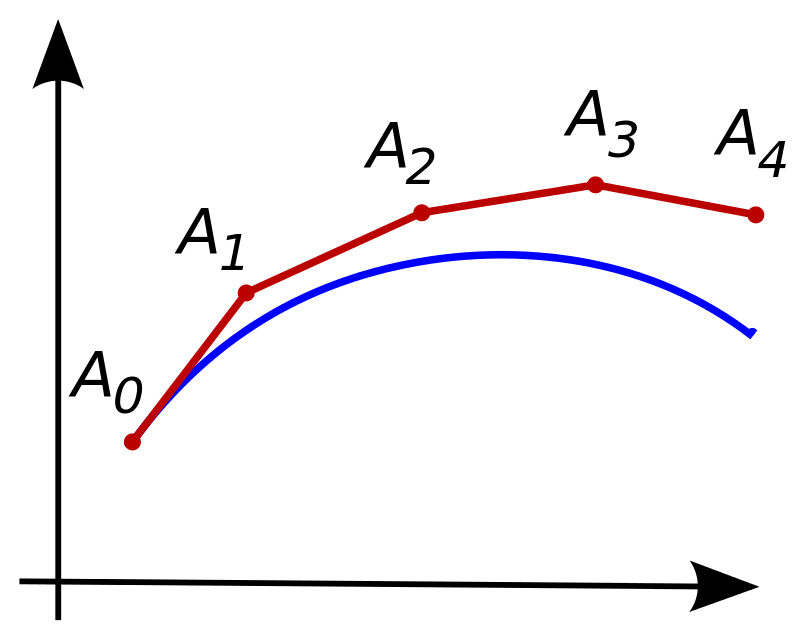
\includegraphics[scale=0.3]{./images/node/euler_method.png}
\end{figure}

\paragraph{Advantages:}
\begin{itemize}
	\item Simple to understand and implement.
	\item Requires only basic arithmetic operations.
\end{itemize}
\paragraph{Disadvantages:}
\begin{itemize}
	\item Low accuracy for large step sizes.
	\item Can become unstable if the step size is not chosen appropriately.
	\item Errors accumulate over time, leading to less accurate solutions.
\end{itemize}

Euler's method is often used as a basic introduction to numerical methods for solving ODEs, and more sophisticated methods like the \textit{Runge-Kutta} methods are used for more accurate solutions.



\section{Neural ODE}


Models such as residual networks, recurrent neural network decoders, and normalizing flows build complicated transformations by composing a sequence of transformations to a hidden state:
$$\rvh_{t+1} = \rvh_{t}+f(\rvh_{t}, \theta_t).$$

The $\rvh$ is iteratively updated as follows:
\begin{align*}
	\rvh_{2} &= \rvh_{1}+f(\rvh_{1}, \theta)\\
	\rvh_{3} &= \rvh_{2}+f(\rvh_{2}, \theta) = \rvh_{1}+f(\rvh_{1}, \theta)+f(\rvh_{2}, \theta)\\
	\vdots
\end{align*}
These iterative update can be seen as \textit{Euler discretization} of the \textit{continuous} transformation. Think of traditional neural networks as a sequence of steps. You give it some input, it goes through several steps (layers), and you get an output. Instead of thinking in steps, Neural ODEs think in \textbf{continuous change over time}. Note that this is the key contribution of this approach.   

Euler method can be expressed as follows: 
$$y_n = y_{n-1}+h\frac{\partial y_{n-1}}{\partial x_{n-1}},$$
where $h$ is the step size. In NODE, they view the $f$ as an ordinary differential equation, which depends on the state at time $t$ and parameter $\theta$. The following equation is the shape of Euler method:
$$y_n = y_{1}+h\frac{\partial y_{1}}{\partial x_{1}}+h\frac{\partial y_{2}}{\partial x_{2}}+\cdots+h\frac{\partial y_{n-1}}{\partial x_{n-1}}.$$
In NODE, 



